\subsection{Computing Bundle Summaries}
\label{sec:bundles_summary}

Intuitively, the first visualization method displays the bundle summaries for a spatial area of interest, as defined in Section~\ref{subsec:bundle_sums}. This may concern the currently visible area on a map, so a set of time series patterns and their respective spatial extents are computed and visualized. Using this process, a user can select the bundle of her preference and the proper spatial summary will appear on the map after acquiring the necessary MBRs from the \btsr index. Whenever the user zooms in/out or pans around the map, the \btsr is traversed, and the corresponding bundles, MBRs, and object counts are obtained to drive the visualization. In each case, the rectangle corresponding to the visible part of the map is used to feed a traversal algorithm that efficiently gathers the results. Next, we first outline the structure of the \btsr index, and then we introduce a novel algrorithm for its traversal in order to compute the bundle summaries for a given area of interest.




\subsubsection{The \btsr Index}
\label{subsec:btsr}

To generate efficient visualizations of geolocated time series data, we need early access to both spatial and time series related information while traversing the index, in order to maintain low latency levels when drawing the required graphic elements. However, none of the approaches presented in Section~\ref{sec:related} supports geolocated time series indexing. To the best of our knowledge, the recently proposed \btsr index \cite{chatzig17btsr} is the only one that provides the desired functionality. 

The \btsr is based on the R-tree \cite{Guttman1984} for the spatial indexing part. The R-tree organizes a hierarchy of nested $d$-dimensional rectangles. Each node corresponds to a disk page and represents the MBR of its children or, for leaf nodes, the MBR of its contained geometries. The number of entries per node (excluding the root) is between a lower bound $m$ and a maximum capacity $M$. Query execution in R-trees starts from the root. MBRs in any visited node are tested for intersection against the search region. Qualifying entries are recursively visited until the leaf level or until no further overlaps are found. Several paths may be probed, as multiple sibling entries could overlap with the search region. The \btsr extends the information stored within each node of the R-tree with bundles of MBTS, as illustrated with the colored strips per node in Figure~\ref{fig:trees}. This allows to efficiently prune the search space when evaluating hybrid queries combining time series similarity with spatial proximity.

A \btsr is constructed exactly like an R-tree \cite{Guttman1984} with respect to the spatial contents of a geolocated time series dataset $\mathcal{T}$, as depicted in Figure~\ref{subfig:example}. As in R-trees, each node of the \btsr has at least $m$ and at most $M$ entries and stores the MBRs of its children. Additionally, for each child, a node stores a pre-specified number of MBTS, shown as colored strips per node in Figure~\ref{subfig:btsrtree}, each one enclosing all the time series indexed in its subtree. Each MBTS is calculated according to Eq.~\ref{eq:bounds1}. Construction and maintenance of the \btsr follow the procedures of the R-tree for data insertion, deletion and node splitting. Objects (i.e., geolocated time series) are inserted into leaf nodes and any resulting changes are propagated upwards.

Once the nodes have been populated, the MBTS of each node are calculated bottom-up. First, in each leaf node, the contained time series are clustered into $k$ bundles using $k$-{\em means clustering} according to their Euclidean distance in the time series domain. Then, the MBTS of each bundle is computed and stored in the node. The example in Figure~\ref{fig:example_bundle} depicts the $k=2$ MBTS (as two bands with a thick outline) obtained for a set of time series (shown as thin polylines). As a next step, each parent node receives all the MBTS of its children and computes its own $k$ bundles and respective set of MBTS by clustering them. The process continues upwards, until reaching the root of the tree. Optionally, \emph{Piecewise Aggregate Approximation} \cite{keogh2001paa,faloutsos2000vldb} can be applied over the time series. As detailed in \cite{chatzig17btsr}, this allows a trade off between the number of bundles per node and the MBTS resolution, thus permitting a larger number ($>k$) of bundles in nodes at higher levels in the tree hierarchy.



\begin{figure}[!t]
 \centering
 \subfloat[Sample dataset with MBRs.]{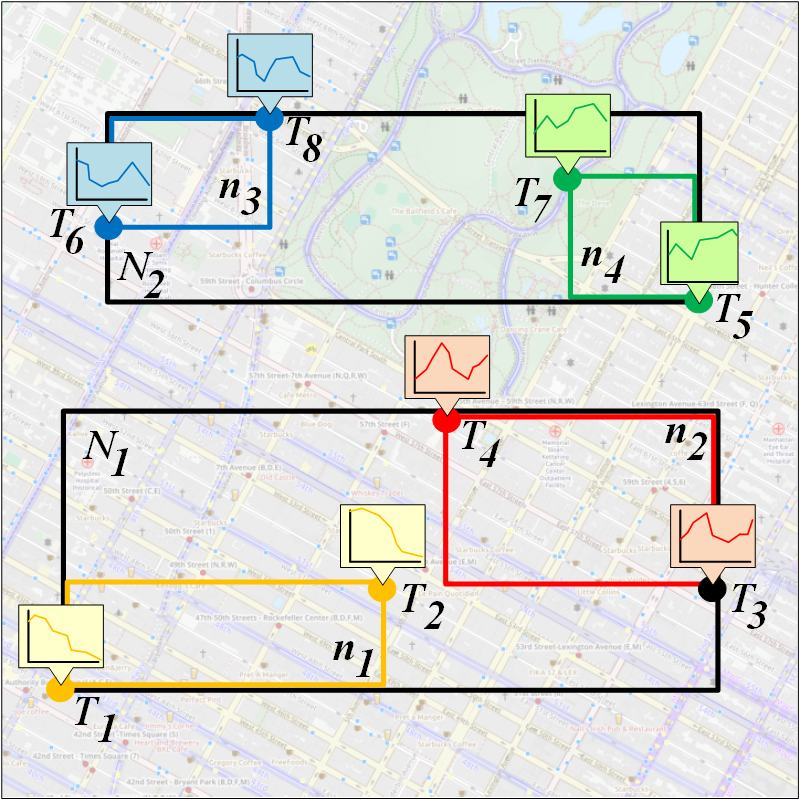
\includegraphics[width=0.5\textwidth]{figures/geotimeseries.png}\label{subfig:example}}
 \subfloat[Hybrid \btsr index.]{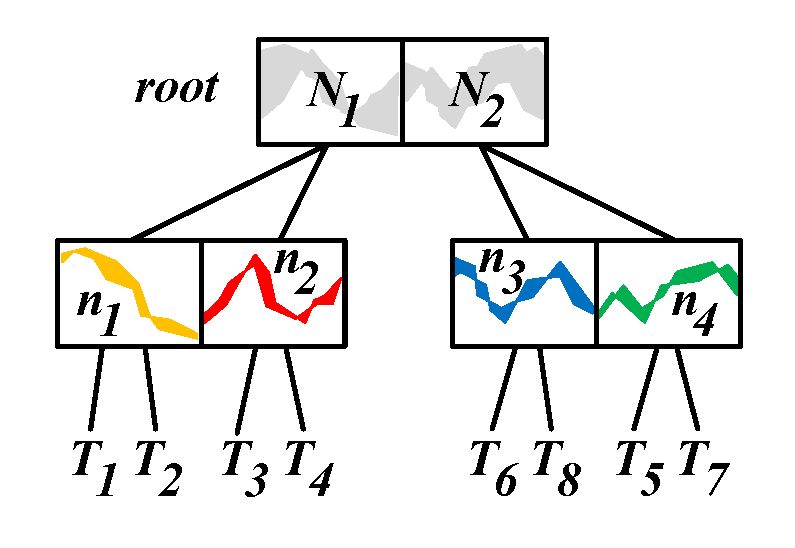
\includegraphics[width=0.45\textwidth]{figures/btsr_tree.pdf}\label{subfig:btsrtree}}\
\caption{Sample dataset with MBRs as maintained by the \btsr index.}
\label{fig:trees}
\end{figure}



\subsubsection{Deriving Bundle Summaries from the \btsr Index}
\label{subsec:visualization}

To support the summaries required by the visualization method, we further extend the information stored in each node of the \btsr index with the {\em count} of geolocated time series that are fully contained within each bundle. This is done bottom-up during insertion, while the index is traversed to calculate the bundles. At each leaf node, after the clustering, we propagate the number of members of each cluster to its parent, which in turn calculates its clusters and aggregates the counts it has received for each bundle's members. This procedure continues up to the root of the tree. We stress that this process concerns the building of the index and is carried out once geolocated time series are being inserted.


We now present our summarization technique for producing map-based visualizations of geolocated time series. The process is outlined in Algorithm~\ref{alg:algorithm1}. It takes as input the {\em input rectangle} $q$, i.e., the spatial area of interest for which the visualization is produced, the number $k$ of bundles and the number $l$ of MBRs per bundle  to be generated. The process comprises three distinct steps. Initially, the \btsr index is traversed to obtain the MBRs contained in the input rectangle, along with their bundles and the number of objects per bundle (Line 1). Next, $k$-means clustering is applied using the average time series per bundle as centroids (Line 2). Finally, the new bundles are calculated and the proper MBRs and corresponding object counts are assigned to each bundle (Line 3). Next, we describe each step in more detail.

\vspace{3mm}

\emph{Step 1: \btsr Traversal}.
During this step, the \btsr index is traversed, with the target being the fast provision of a predefined number $k$ of geolocated time series bundles contained within the given area $q$, along with $l$ MBRs where these bundles can be found and the total number of geolocated time series that reside within each MBR. All required information is stored within the nodes of the \btsr, thus, when a node that is contained within the input rectangle is found, the relevant information is retrieved and added to the intermediate results, without any need to continue searching in its sub-tree. The output of this step is passed to the next phase of bundle clustering. 

In more detail, the traversal is performed as follows. After initializing a queue with the root's children (Line 7), we iterate over it (Line 8) until it is empty. For each inner node's child $N'$, we check whether its MBR is contained within the given input rectangle $q$ (Lines 11--12). If so, its MBR, the time series bundles, and the number of objects per bundle are added to the intermediate results (Line 13) as a {\em tuple} with the following components:

\begin{equation*}
\langle mbr, \{ (mbts_1,cnt_1), ..., (mbts_k, cnt_k) \} \rangle.
\end{equation*}

\noindent Each such tuple indicates the MBR of a node ($mbr$), consisting of the coordinates of the lower left and upper right point, as well as $k$ pairs denoting the bundles of the node along with the corresponding number of objects per bundle. If the MBR is not contained in the input rectangle $q$, we check whether it overlaps with $q$ and if so, we add the child node to the queue (Line 15). If not, this MBR is located outside the input rectangle, and thus we can skip searching this subtree. Once no more nodes are left to search, the intermediate results are finally returned (Line 16).

\vspace{3mm}

\emph{Step 2: Bundles Clustering}.
The aforementioned traversal method returns tuples, each containing the bundles residing in the input rectangle, the corresponding nodes' MBRs and the number of objects per bundle. Next, $k$-means clustering is executed on the average time series of each bundle. Line 2 of Algorithm~\ref{alg:algorithm1} calls the clustering procedure. Initially, for each tuple (Line 20), we iterate over its bundles (Line 21) and generate a new tuple per bundle of the following format: 
\begin{equation*}
\langle T_{avg}, mbts, cnt, mbr \rangle
\end{equation*}

\noindent This new tuple contains an average time series, the bundle itself ($mbts$), the number $cnt$ of objects enclosed in this bundle, and the MBR ($mbr$) this bundle belongs to (Line 23). The average time series $T_{avg}$ is calculated by averaging the upper and lower bound of each bundle (Line 22), i.e., average value at each time point. The resulting collection of tuples is fed to the $k$-means algorithm (Line 24) in order to return the required number $k$ of bundles to be created. This clustering generates a clustered collection of tuples using the calculated average time series. These results are then forwarded to step 3 (Line 25).

\vspace{3mm}

\emph{Step 3: Bundles Calculation and MBR Assignment}.
During this step, the clustered tuples received from step 2 are used to calculate the final bundles, the corresponding $l$ MBRs and total number of objects per MBR are assigned to each bundle. The final bundles are calculated in a similar manner to the MBTS bundles during \btsr construction. More specifically, at each time point, we obtain the maximum and minimum value among the corresponding upper and lower bounds for the bundles of each cluster (see Section \ref{subsec:btsr}). Then, we apply $k$-means clustering on each bundle's MBRs, obtaining a total of $l$ new MBRs per bundle along with an aggregate count of the time series contained therein. The final result is then used for visualization.

Line 3 of Algorithm~\ref{alg:algorithm1} calls the corresponding procedure. For each cluster of tuples received from step 2 (Line 28), we loop over its members (Line 31) and we use each tuple's bundle to update the upper and lower bounds (Line 32). Then, we apply $k$-means clustering on the cluster's MBRs, obtaining $l$ new MBRs along with their counts (Line 33). Once the bounds and the corresponding list of MBRs for the current bundle have been calculated, we issue an aggregated tuple to the final result (Line 34). This tuple has the following components:

\begin{equation*}
\langle mbts', \{ (mbr_1,cnt_1), ..., (mbr_l, cnt_l) \} \rangle
\end{equation*}

\noindent where $mbts'$ is a resulting bundle, along with $l$ MBRs associated with it. Each MBR is accompanied with the corresponding number of objects (i.e., raw time series) therein. The final result with all such tuples is then returned in order to generate the visualization (Line 36).

\begin{algorithm}[!ht]
	\DontPrintSemicolon
	\KwIn{Input rectangle $q$; number $k$ of bundles to be generated; number $l$ of MBRs per bundle}
	\KwOut{A list $R_{b}$ containing tuples of bundles, MBRs, and object counts}
	$R \leftarrow IndexTraversal(q)$   \tcp*{Step 1}
	$R_{c} \leftarrow BundlesClustering(R, k)$   \tcp*{Step 2}
	$R_{b} \leftarrow BundlesCalculation(R_{c}, l)$   \tcp*{Step 3}
	\KwRet $R_{b}$ \\
	\vspace{3pt}
	\SetKwProg{procTraversal}{Procedure}{}{}
	\procTraversal{$IndexTraversal(q)$}{
		$R \leftarrow \emptyset$ \\
		$Q \leftarrow Root.getChildren()$ \\
		\While{$Q \neq \emptyset$}{
			$N \leftarrow Q.getNext()$ \\
			\If{$N$ is not leaf}{
				\ForEach{$N' \in N.getChildren()$}{
					\If{$q.contains(N'.mbr)$}{
						\mbox{$R \leftarrow R \cup \{\langle N'.mbr, \{(N'.mbts, N'.cnt)\} \rangle\}$} \\
					}
					\ElseIf{$q.overlaps(N'.mbr)$}{
						$Q \leftarrow Q \cup N'.getChildren()$
					}
				}
			}
		}
		\KwRet $R$ \\
	}
	\vspace{3pt}
	\SetKwProg{procCluster}{Procedure}{}{}
	\procCluster{$BundlesClustering(R, k)$}{
		$R_{c} \leftarrow \emptyset$ \\
		$C \leftarrow \emptyset$ \\
		\ForEach{$t \in R$}{
			\ForEach{$b \in t.mbts$}{
				$T_{avg} \leftarrow avg(b.up, b.lo)$ \\
				$C \leftarrow C \cup \{\langle T_{avg}, b, t.cnt(b), t.mbr \rangle\}$ \\
			}
		}
		$R_{c} \leftarrow kmeans(C.avg, k)$ \\
		\KwRet $R_{c}$
	}
	\vspace{3pt}
	\SetKwProg{procBundles}{Procedure}{}{}
	\procBundles{$BundlesCalculation(R_{c}, l)$}{
		$R_{b} \leftarrow \emptyset$ \\
		\ForEach{$Cl \in R_{c}.clusters$}{
			$mbts \leftarrow \emptyset$ \\
			$mbr \leftarrow \emptyset$ \\
			\ForEach{$t \in Cl$}{
				$mbts \leftarrow updateMBTS(mbts, t.mbts)$ \\
				$ \{(mbr, cnt)\} \leftarrow kmeans(l, t.mbr, t.cnt)$ \\
			}
			$R_{b} \leftarrow R_{b} \cup \{\langle mbts,  \{(mbr, cnt)\} \rangle\} $ \\
		}
		\KwRet $R_{b}$
	}
	\caption{Bundles Summarization of Geolocated Time Series}
	\label{alg:algorithm1}
\end{algorithm}